\documentclass[12pt,a4paper]{article}
\usepackage[swedish]{babel} %göra så att autogenererade saker blir på svenska
\usepackage[T1]{fontenc} %rendera åäö bättre
\usepackage[utf8]{inputenc} %använda utf-8
\usepackage[parfill]{parskip} %gör så att styckena blir den "rätta" sorten
\usepackage{mathtools}
\usepackage{listings}
\usepackage{algorithm}% http://ctan.org/pkg/algorithms
\usepackage{algpseudocode}% http://ctan.org/pkg/algorithmicx
\newcommand{\var}[1]{{\ttfamily#1}}% variable

\usepackage{hyperref}
\def\fpage{\pageref{CorrectFirstPageLabel}} % fixar en bugg i hyperref

\usepackage[nottoc,numbib]{tocbibind} %få references in table of contents

\usepackage{float}
\floatstyle{boxed} 
\restylefloat{figure}

\title{Jämförelse av skräpsamlingsmetoder}
\author{Erik Rimskog}
% \date{}

\begin{document}
\pagenumbering{gobble}
\maketitle
\pagebreak
\pagenumbering{arabic}
\tableofcontents

\pagebreak

\section{Inledning}
\label{sec:inledning}

\subsection{Syfte}
\label{subsec:syfte}

Denna uppsats ska jämföra två metoder av skräpsamling, nämligen ``mark
and sweep'' och ``generational GC''. Båda metoderna kommer att
förklaras på en hög abstraktionsnivå, hur de fungerar, dessutom kommer
deras för- och nackdelar att tas upp och jämföras.

\subsection{Bakgrund}
\label{subsec:gc}

När man programmerar i programspråk som har manuell minneshantering så
som C eller C++ måste man manuellt allokera och frigöra minne för sina
objekt. Det kan vara svårt att veta när och var ett objekt ska
frigöras. Samt så kan det leda till många olika sorters jobbiga buggar
och problem. Exempelvis aliaseringsproblem då två olika pekare pekar
på samma objekt och en av dem frigör objektet. Den andra pekaren
kanske förväntar sig att objektet fortfarande finns och försöker att
avreferera den.

För att automatisera detta finns skräpsamlare (\textit{eng}. garbage
collector, \textit{förkortat}. GC), som är en rutin som körs i
bakgrunden av det nuvarande programmet. Skräpsamlaren går igenom
minnet vid vissa tillfällen för att söka efter objekt som inte längre
används för att frigöra dem.

\pagebreak

\section{Skräpsamlingsmetoder}
\label{sec:main}

De två metoder som skall jämföras är ``Mark and Sweep'' och
``Generational Garbage Collector''. Båda bygger på samma princip; att
stanna programmet (sk. ``Stop the world'') för att söka minnet. Det
finns en annan metod, ``Reference Counting'', som kollar minnet
samtidigt som programmet ändrar i det. Men den kommer inte att tas upp
här.

Observera att \underline{när} en skräpsamlare väljer att stanna upp
programmet beror helt på implementationen. Det kan vara att den körs
när minnet är fullt, vid olika tidsintervall eller något helt annat.
Så det är inte alls bestämt om när skräpsamling körs och det kan variera
mycket.

\subsection{Mark and Sweep}
\label{subsec:marksweep}

Det mest simpla sättet att göra en mark and sweep-algoritm på är att;
stanna hela programmet, skanna minnet och markera alla objekt som kan
nås (mark), för att till sist gå igenom minnet och ta bort alla objekt
som inte blev markerade (sweep).

\subsubsection{Mark}
\label{subsec:mark}

För att markera objekt åstadkoms detta genom att ge alla objekt en bit
som representerar om objektet kan nås eller inte. Ett objekt kan nås
om:

\begin{itemize}
  \item den är refererad från en ``root'' (objekt som vi vet kan nås. Så som variabler på stacken eller globala variabler)
  \item den är refererad från ett annat nåbart objekt
\end{itemize}

\bigskip

Psuedokod för en mark-fas kan se ut på förljande vis:

\begin{algorithm}[H]
  \caption{Mark-algoritmen}\label{markalg}
  \begin{algorithmic}[1]
    \State \var{todo} $\gets$ $\{$ alla roots $\}$ 
    \While{\var{todo} $\not= \emptyset$}
      \State let $u \in$ \var{todo}
      \State \var{root} $\gets$ \var{root} $\setminus$ $\{u\}$
      \If{mark($u$) $=$ 0}
        \State mark($u$) $\gets 1$
        \State let $\{v_0, v_1 \ldots v_n \}$ vara alla referenser i $u$
        \State \var{todo} $\gets$ \var{todo} $\cup \ \{v_0, v_1 \ldots v_n \}$
        \EndIf
    \EndWhile\label{euclidendwhile}
  \end{algorithmic}
\end{algorithm}

På rad~1 skapas en lista där alla objekt som ännu inte har sökts
igenom lagras. Sedan i loopen på rad~2-10 itereras alla objekt tills
det inte finns några kvar att söka igenom. I varje iteration av loopen
plockas ett objekt $u$ ut ur listan (rad~3-4). Om $u$ inte tidigare
blivit markerad (rad~5) så markeras den (rad~6), annars går vi vidare
med nästa objekt. Om $u$ inte var markerad läggs alla objekt som $u$
kan nå till i listan för att genomsökas (rad~7-8).

\begin{figure}[H]
  \centering
  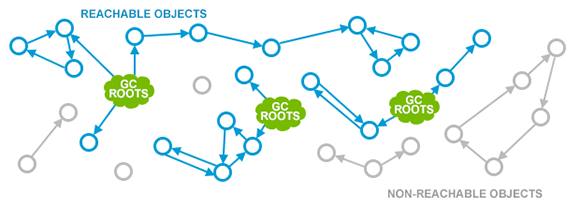
\includegraphics[width=1\textwidth]{mark_and_sweep.png}
  \caption{exempel på en körning av mark-algoritmen (alg~\ref{markalg}). De blåa cirklarna är objekt som har blivit markerade och fortfarande används, de grå är omarkerade objekt och är redo att bli skräpsamlade. Bild från \cite{plumbr1}}
  \label{fig:alg1}
\end{figure}

\subsubsection{Sweep}
\label{subsec:sweep}

Efter en markeringsfas (som beskrivs i \ref{subsec:mark}) kommer
sweep-fasen. I denna fas skannas hela arbetsminnet och varje objekts
markeringsbit kollas. Om den är satt återställs bit:en, om den inte är
satt frigörs objektet.

Ett problem med detta är att minnet antagligen kommer att bli
fragmenterat (översta raden på figur~\ref{fig:frag}). Detta leder till
att det kan bli svårt att allokera minne till nya objekt. För att
allokera nya objekt måste det finnas någon sorts lista som har pekare
till alla lediga block. När ett objekt ska allokeras kommer de lediga
blocken att kontrolleras en efter en tills man hittar ett block som
objektet får plats i. Fragmenteringen kan till och med göra att det
inte finns ett tillräckligt stort ledigt block kvar för ett nytt
objekt, även fast den totala mängden ledigt arbetsminne är
tillräcklig.

En lösning till detta fragmenteringsproblem är att kopiera de objekt
som inte blev frigjorda bredvid varandra till ett stort kontinuerligt
block (se den undre raden på figur~\ref{fig:frag}), detta brukar
kallas för mark-compact. Detta löser problemet för att nu är det
trivialt att allokera nytt minne, det är bara att flytta fram en
pekare som pekar där det lediga arbetsminnet börjar. Nackdelen att
göra på detta sätt är att massor av tid spenderas på att kopiera
objekt.

\begin{figure}[H]
  \centering
  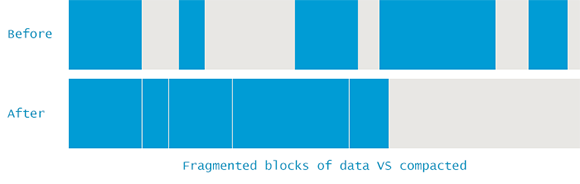
\includegraphics[width=1\textwidth]{frag_vs_comp_mem.png}
  \caption{översta raden är exempel på fragmenterat minne, medan den undre raden visar hur ett komprimerat minne ser ut. Bild från \cite{plumbr2}}
  \label{fig:frag}
\end{figure}

\subsection{Generational GC}
\label{subsec:generational}

Generational Garbage Collector (GGC) försöker att vara mer effektiv än
mark and sweep (se~\ref{subsec:marksweep}) genom att utgå ifrån
att de flesta objekt som skapas antingen lever en väldigt lång tid,
eller en väldigt kort tid. Den använder sig utav detta genom att skapa
``generationer'', några för de som har ett kort liv och en för de som
har ett långt liv. Generationerna som skapas är: \textit{Eden},
\textit{Surivor 1}, \textit{Surivor 2}, \textit{tenured} och
\textit{permgen}. Poängen med generationerna är att inte behöva
skräpsamla hela minnet på samma gång, utan bara en del av den åt gången.

\begin{figure}[H]
  \centering
  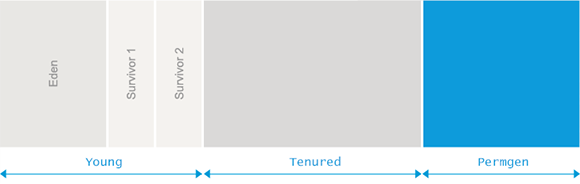
\includegraphics[width=\textwidth]{ggc_generations.png}
  \caption{\label{fig:generations} Illustration på alla generationer. Bild från \cite{plumbr2}}
\end{figure}

\subsubsection{Den unga generationen}
\label{subsubsec:young}

Alla nya allokeringar av objekt kommer att hamna i eden. När eden blir
full kommer den unga generationen att skräpsamlas. Då markeras alla
objekt som kan nås, precis som i mark and sweep (\ref{subsec:mark}).
Den stora skillnaden är att istället för att följa och markera
referenser genom hela minnet begränsar vi oss bara till eden och
survivor 1 och 2. Alltså om en referens skulle leda till den gamla
generationen slutar vi helt enkelt att följa den. Problemet är dock om
ett objekt i eden inte kan nås direkt ifrån en root, utan endast
indirekt från ett objekt i den gamla generationen, kommer det objektet
inte att markeras och kommer att skräpsamlas fastän den fortfarande
lever. Detta kan man lösa med t.ex. card marking, vilket inte kommer
att tas upp här.

Survivor-sektionerna är lite speciella, en kallas för \textit{to}
(denna är alltid tom) och en för \textit{from} (här finns levande
objekt). När markeringsfasen är klar kommer alla levande objekt från
eden och en utav survivor-sektionerna (\textit{from}) att kopieras
till den andra survivor-sektionen (\textit{to}). Nu anses eden och
\textit{from} som tomma och survivor-sektionerna byter roll till nästa
skräpsamlingsfas. Observera att objekten i survivor inte är
fragmenterade, då de kopieras och hamnar i ett kontinuerligt block.

\begin{figure}[H]
  \centering
  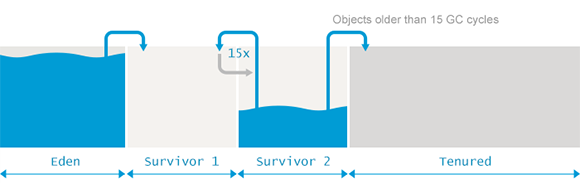
\includegraphics[width=\textwidth]{ggc_survivor.png}
  \caption{\label{fig:survivor} Denna bild illustrerar hur objekt flyttas mellan sektionerna}
\end{figure}


Varje gång objekten kopieras fram och tillbaka mellan
survivor-sektionerna ökas en räknare för varje objekt. När ett objekts
räknare överstiger ett visst värde kommer det objektet att kopieras
till \textit{tenured} istället för den andra survivor-sektionen. Ett
sådant objekt har levt ett långt tag och förväntas att leva väldigt
länge, därför uppgraderas dessa till den gamla generationen. 

\subsubsection{Den gamla generationen}
\label{subsubsec:gamla}

Skräpsamling i den gamla generationen händer inte lika ofta då objekten
förväntas leva länge. Metoden för att skräpsamla i \textit{tenured}
(se bild~\ref{fig:generations}) är mark-compact som är beskriven
i detalj i sektion~\ref{subsec:sweep}.

I den gamla generationen finns också en sektion som kallas för
\textit{permgen}. Här lagras data om själva programmet så som klasser.
Detta utrymme kommer aldrig att skräpsamlas.

\pagebreak
\section{Jämförelse}
\label{sec:compare}

Vilken metod som är bäst beror på vad för sorts program de används till.
Eftersom mark and sweep stannar upp hela programmet för att skräpsamla
hela minnet är nog denna metod inte så passande att ha i ett
interaktivt program så som spel. Att ha spelet frysa lite då och då
för att skräpsamla gör nog att spelet inte blir så kul att använda och
kan kännas långsamt. Denna metod är dock mycket enklare att
implementera och är kanske snabbare än Generational GC om man inte
behöver skräpsamla så ofta.

Generational GC (GGC) är mer komplicerad men är generellt snabbare än
mark and sweep. GGC är optimerad för program som skapar många objekt
som inte lever så länge. De allra flesta program beter sig på detta
vis, så därför är GGC väldigt bra. GGC gör inga gigantiska pauser för
att skräpsamla, utan den gör flera mindre pauser istället. Det är bra
för då får man inga märkbara pauser, men istället kan den totala tiden
som skräpsamlaren använder vara större än om man gör få stora pauser.

Mark and sweep gör så att minnet blir fragmenterat och man måste
använda alternativa metoder så som mark-compact för att åtgärda det.
GGC har däremot av design defragmentering inbyggt då den alltid
kopierar alla objekt när den skräpsamlar. Detta gör att enkel mark and
sweep är snabbare än GGC, men eftersom allokering av nya objekt blir
mycket svårare är GGC bättre.

\pagebreak

\begin{thebibliography}{9}

  \bibitem{wikipedia1}
  Wikipedia,
  \textbf{Garbage collection (computer science)},
  \url{https://en.wikipedia.org/wiki/Garbage_collection_(computer_science)}

  \bibitem{wikipedia2}
  Wikipedia,
  \textbf{Tracing garbage collection},
  \url{https://en.wikipedia.org/wiki/Tracing_garbage_collection}

  \bibitem{plumbr1}
  Plumbr.io,
  \textbf{What is Garbage Collection},
  \url{https://plumbr.io/handbook/what-is-garbage-collection}

  \bibitem{plumbr2}
  Plumbr.io,
  \textbf{Garbage Collection in Java},
  \url{https://plumbr.io/handbook/garbage-collection-in-java}

\end{thebibliography}

\end{document}